\chapter{Project Schedule \& Resources Allocation} \label{chap4}
In defining the possible schedule for the project we have tried to adhere as much as possible to the result of the previous evaluation made using FP and COCOMO II adapting those prescriptions to our specific case (a team composed of 3 people).
We have identified 6 major tasks to carry out during the development of the project:
\begin{itemize}
	\item T1 : Feasibility study
	\item T2 : Analysis of Requirements and specifications
	\item T3 : Design of the system
	\item T4 : Coding and Unit testing
	\begin{itemize}
		\item T4.1 : Client Side
		\item T4.2 : Server Side
		\item T4.3 : Database
	\end{itemize}
	\item T5 : Integration test and system test
	\item T6 : Deployment
\end{itemize}
In the effort of balancing as much as possible the workload of each component of the team we have developed the following Gantt diagram (Figura \ref{fig:scheduele}) showing the distribution of every task among the team members during the months, forecasting a total duration of 10 months (rounding down with respect to the prescription obtained using COCOMO II to balance the dimension of the team - 3 people instead of 2,38).

\begin{figure}[!htbp]
\centering
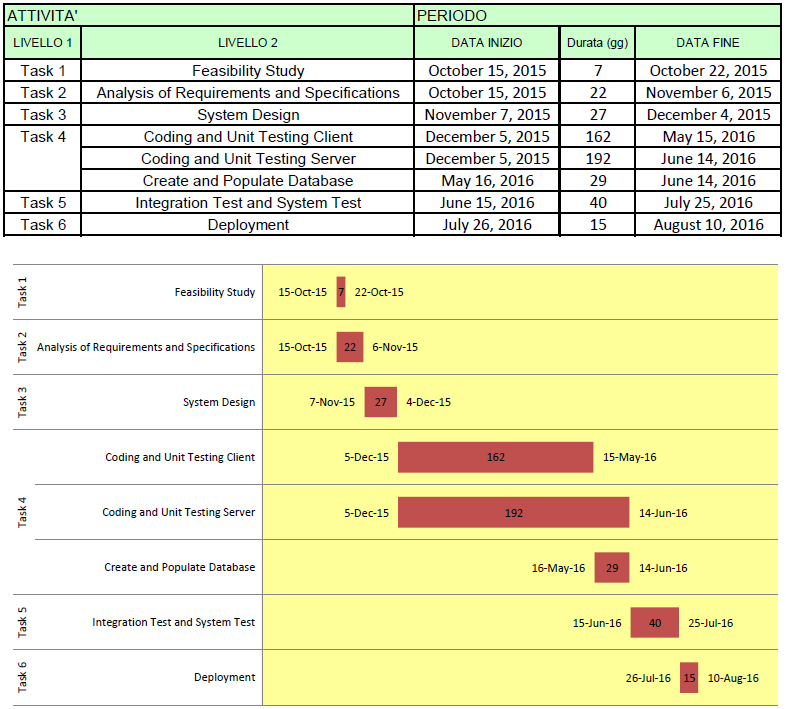
\includegraphics[width=\textwidth]{cpt/img/Schedule}
\caption{Project schedule}
\label{fig:scheduele}
\end{figure}